\documentclass{article}
\usepackage{amsmath}
\usepackage{ctex}
\usepackage{graphicx}

\begin{document}
	The Lorenz system:
	\begin{displaymath}
		\left\{\begin{array}{l}
		\dot{x} = -\sigma x + \sigma y\\
		\dot{y} = \gamma x - y -xz \\
		\dot{z} = xy - bz
		\end{array}
		\right.
	\end{displaymath}
	
	Jacobian:
	\begin{displaymath}
		\mathbf{J}=
		\left(\begin{array}{ccc}
		-\sigma & \sigma & 0 \\
		\gamma-z & -1 & -x \\
		y & x & -b 
		\end{array}
		\right)
	\end{displaymath}
	
%------Parameter array 1
\section{Parameter set 1}	
	\begin{table}[!hbp]
	\caption{The complete set of Lyapunov exponent for the Lorenz system with $\sigma=10,b=8/3,\gamma=28$. The column of values are given by Liao 2008.}
		\begin{tabular}{|l|l|}
		\hline
			$\lambda_1$ & 0.91 \\
		\hline
			$\lambda_2$ & 0 \\
		\hline
			$\lambda_3$ & -144.47\\
		\hline
		\end{tabular} 
	\end{table}
	
	\begin{figure}[!hbp]
	\centering
	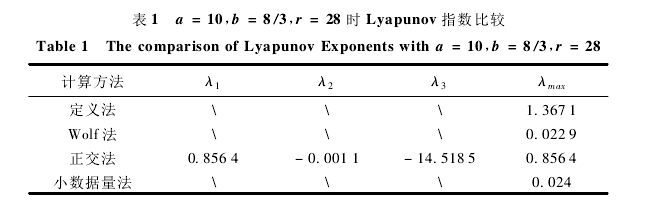
\includegraphics[width=1.4\linewidth]{./zhang2012}
	\caption{Calculating LE with different methods}
	\label{fig:zhang2012}
	\end{figure}	
	
	\begin{figure}[!hbp]
	\centering
	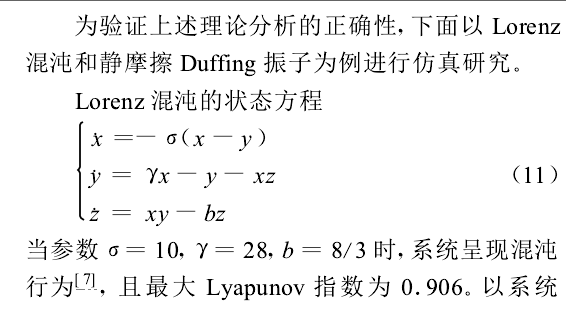
\includegraphics[width=1.2\linewidth]{./yang}
	\caption{}
	\label{fig:yang}
	\end{figure}

%------Parameter array 2
\section{Parameter set 2}
	\begin{table}[!hbp]
	\caption{The complete set of Lyapunov exponent for the Lorenz system with $\sigma=16,b=4.0,\gamma=40$. The column of values are given by Shimada 1979.}
		\begin{tabular}{|l|l|}
		\hline
			$\lambda_1$ & 1.37 \\
		\hline
			$\lambda_2$ & 0 \\
		\hline
			$\lambda_3$ & -22.37\\
		\hline
		\end{tabular}
	\end{table}
	
%-----Parameter array 3
\section{Parameter set 3}
	\begin{table}[!h]
	\caption{The complete set of Lyapunov exponent for the Lorenz system with $\sigma=16,b=4.0,\gamma=45.92$. The second column is given by A. Wolf 1980,while the third column is given by Kehui Sun 2004.}
		\begin{tabular}{|l|l|l|}
		\hline
			$\lambda_1$ & 2.16 & 1.506 \\
		\hline
			$\lambda_2$ & 0.00 & 0.001 \\
		\hline
			$\lambda_3$ & -32.4 & -22.505\\
		\hline
		\end{tabular}
	\end{table}
	
	\begin{figure}
	\centering
	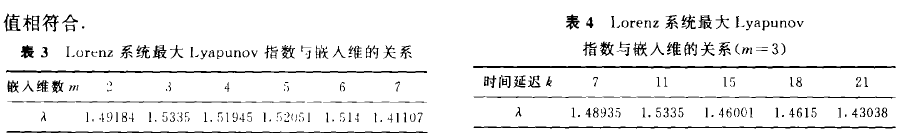
\includegraphics[width=1.2\linewidth]{./Li2003}
	\caption{LLE for the Lorenz system with parameter $\sigma=16,b=4.0,\gamma=45.92$}
	\label{fig:Li2003}
	\end{figure}

\end{document}